\documentclass[12pt,openany,twoside,a4paper]{article}
\usepackage{amsmath}
\usepackage{amssymb}
\usepackage{geometry}
\usepackage{fancyhdr}
\usepackage{hyperref}
\usepackage{cleveref}
\usepackage{graphicx}
\usepackage{subcaption}
\usepackage{esint}
\usepackage{eucal}
\usepackage{float}
\usepackage{pgfplots}
\usepackage[dvipsnames]{xcolor}
\usepackage{listings}
\usepackage[italian,english]{babel}
\usepackage[utf8]{inputenc}

\usepackage[
backend=biber, style=numeric, sorting=nyt]{biblatex}
\addbibresource{bibtex.bib}

\selectlanguage{italian}

\definecolor{light-gray}{gray}{0.85}
\definecolor{dark-green}{RGB}{0,100,0}
\newcommand{\code}[1]{\colorbox{light-gray}{\texttt{#1}}}

\lstdefinestyle{mystyle}{
    backgroundcolor=\color{light-gray},   
    commentstyle=\color{dark-green},
    keywordstyle=\color{magenta},
    numberstyle=\tiny\color{black},
    stringstyle=\color{blue},
    basicstyle=\ttfamily\footnotesize,
    breakatwhitespace=false,         
    breaklines=true,                 
    captionpos=b,                    
    keepspaces=true,                 
    numbers=left,                    
    numbersep=5pt,                  
    showspaces=false,                
    showstringspaces=false,
    showtabs=false,                  
    tabsize=2
}

\lstset{style=mystyle}

\newtheorem{defn}{Definition}
\newtheorem{theom}{Theorem}
\newtheorem{prop}{Proposition}
\newtheorem{exmp}{Example}

\begin{document}

\thispagestyle{empty}
\begin{center}\textsc{\Large POLITECNICO DI TORINO}

\vspace{1cm}
\large{Corso di Laurea Magistrale in Ingegneria Matematica}

\vspace{1.5cm}
\begin{figure}[h]
  \centering
  
\includegraphics[keepaspectratio,height=4cm]{logo.png}
\end{figure}
\vspace{1.5cm}
\textbf{\Large Technical report:}

\vspace{0.25cm}
\Large settings and performances of DiSMA on test cases

\vspace{7.5cm}
\large Davide Papapicco
\end{center}

\pagenumbering{gobble}

\cleardoublepage

\textbf{\large{DISCLAIMER}}
\newline
\newline
At the present release \code{DiSMA-v1.0} the library can only integrate differential problems over $2-$dimensional rectangular domains.
\newpage

 \newgeometry{
 a4paper,
 total={170mm,270mm},
 left=20mm,
 top=10mm,
 }
\section{User interaction with the library}

The present report shows the functionality of \code{DiSMA} (Differential Solver for Matlab Applications) for several parametric formulation of the same test case; the results described in the following sections are associated to the numerical simulations collected in the \code{Tutorials} sub-directory of the library and they follow the same naming convention.
\newline The test cases discussed here all aim to discretise and approximate the analytical solution of a model equation with partial derivatives with parametric and time dependence.
\subsection{$d-$dimensional unsteady model equation}
The PDE is defined over a computational domain $\Omega\subset\mathbb{R}^d$ over which a mesh $\Omega_h$ is introduced for the approximation of the continuous solution; for unsteady problem we will consider the cartesian product $\Omega\times\mathbb{R}^{+}$ as the space-time domain of the problem.
We consider a generic scalar function $u(\mathbf{x},t)$ as the unknown solution of the differential model, whose most general strong formulation as a IBVP associated to the PDE in $d-$dimension, takes the following form (spatial and time dependence is implied for $u(\mathbf{x},t)$ whenever possible for the sake of simplicity)
\begin{equation*}
    \begin{cases}
        \partial_t u- \nabla\cdot(\nu(\mathbf{x},t)\nabla u) + \nabla\cdot(\boldsymbol{\beta}(\mathbf{x},t)u) + \sigma(\mathbf{x},t)u = f(\mathbf{x},t)\;,\quad \forall\mathbf{x}\in\Omega\;,\quad\forall t\in[0,T] \\
        u(\mathbf{x},t) = (g_D(\mathbf{x},t))\;\quad\forall\mathbf{x}\in\Gamma_D \\
        \partial_{\mathbf{\hat{n}}}u := \nabla u(\mathbf{x},t)\cdot\mathbf{\hat{n}} = g_N(\mathbf{x},t))\;,\quad\forall\mathbf{x}\in\Gamma_N\\
        u(\mathbf{x},0) = u_0(\mathbf{x})\;,\quad\forall\mathbf{x}\in\Omega
    \end{cases}\,,
\end{equation*}
where $\nu(\mathbf{x},t)\,,\;\boldsymbol{\beta}(\mathbf{x},t)\,,$ and $\sigma(\mathbf{x},t)$ quantify the relative magnitude of the diffusive, convective and reactive phenomena respectively whereas $f(\mathbf{x},t)$ models the source term function. We denote $\Gamma_D$ and $\Gamma_N$ as the mutually disjoint $(\Gamma_D\cap\Gamma_N = \emptyset)$ portions of the boundary $\partial\Omega$ of the spatial domain over which we set Dirichlet $(g_D(\mathbf{x},t))$ and Neumann $(g_N(\mathbf{x},t))$ boundary conditions (BCs) respectively.
\subsection{Input file}
The structure of DiSMA is s.t. all the information necessary from the user for it to discretise and solve the model equations are passed via a single script called by default \code{Inputs.m} but it can be renamed according to the user preference. One recommended practice for naming the file according to the simulations one is performing; for example if the users wants to run a series of simulations based on the same model but with different parameters then he/she can copy the file as many times as necessary and rename each one in accordance with the modifications made to the parameter functions.
\newline
The information that the user is required to specify are divided in \textbf{explicit} (the user must provide the information by hand) and \textbf{implicit} (the user can select the desired setting among a set of pre-existing selections). The former inputs are:
\begin{itemize}
    \item Coordinates of the input vertices for the domain ($2$ for $1-$dimensional simulations and $4$ for $2-$dimensional simulations);
    \item Explicit functional form of the coefficient $\nu(\mathbf{x},t)$, $\boldsymbol{\beta}(\mathbf{x},t)$, $\sigma(\mathbf{x},t)$ and the source functions $f(\mathbf{x},t)$;
    \item Explicit functional form of the analytical solution $u(\mathbf{x},t)$ and its first order derivative $\nabla u$;
    \item Explicit Dirichlet and Neumann boundary functions $g_D(\mathbf{x},t)$ and $g_N(\mathbf{x},t)$;
    \item Length of simulated time $T>0$ and timestep $\delta t$ for the solution of the associated time-dependent ODE. 
\end{itemize}
The implicit information consist in selecting:
\begin{itemize}
    \item Number of iterations for the grid convergence error estimation \code{Ns} $\in \{2,\:4,\:6,\:8,\:10\}$;
    \item Subspace of the basis function \code{subspace} $\in\{{\mathbb{P}_1,\:\mathbb{P}_2}\}$;
    \item Number of spatial dimensions \code{d} $\in\{{1,\:2}\}$;
    \item Time dependence (unsteady) or independence (stationary) \code{time} $\in\{\text{\textcolor{magenta}{True}},\:\text{\textcolor{magenta}{False}}\}$;
    \item Discretisation algorithm and solver for the time-dependence.
\end{itemize}

An example of the input file is shown below; in it we set the various terms in order to solve the $2-$dimensional test cases discussed below in the present report.
\newpage
\lstinputlisting[language=Matlab]{Inputs.m}

\subsection{Test cases}

In the following sections we will show the outputs of the solver against different instances of the same test case in $1$ and $2$ spatial dimensions.
Since the presence of advective and reactive phenomena directly contirbute to the mesh Peclet number, they have to be set carefully in order to derive accurate and stable simulations; as such, for the sake of simplicity, the test case considered throughout the report will be one of pure-diffusion, i.e. $\boldsymbol{\beta},\sigma = 0\,$, $\nu(\mathbf{x},t)\neq0$.

\subsubsection{$1-$dimensional setting}

\newpage
\subsubsection{$2-$dimensional setting}
We want our solution to be a multivariate normal distribution $e^{\:\frac{1}{2}\mathbf{x}^T\mathbf{x}}$ with the unitary square in the first quadrant of the $x-y$ plane as spatial domain, i.e. $\Omega = [0,1]\times[0,1]$. In order to achieve the desired result we must, given a certain function $\nu(\mathbf{x},t)$ calculate the correct source and boundary functions.
\newline The calculation of the source function we start by computing the spatial partial derivatives of the desired solution and then plug both $\nabla u$ and $u$ in the model equation
\begin{equation*}
    \nabla u = (\partial_xu, \partial_y u)^T = (-2x\,e^{\:(-x^2 - y^2)}, -2y\,e^{\:(-x^2 - y^2)})^T = -2u\begin{pmatrix} x \\ y \end{pmatrix}
\end{equation*}
\begin{equation}\label{eq1}
    f(\mathbf{x},t) = -\nabla\cdot(\nu\nabla u) = -\nabla\nu\cdot\nabla u - \nu\Delta u = 2u\,(\nabla\nu)^T\begin{pmatrix} x \\ y \end{pmatrix}-\nu\Delta u\,,
\end{equation}
and complete the calculation according to $\nu(\mathbf{x},t)$.
\newline The computation for the Dirichlet and Neumann boundary functions is less straightforward and we will refer to the graphical representation of the domain and the analytic function itself. Let's start by considering the Neumann boundary functions as they are somewhat less complicated to derive in a general fashion; as in Figure \ref{geomSquare}, the computational domain of our test case features 4 normal vectors (one for each edge of the domain) which are
\begin{equation*}
    \mathbf{\hat{n}_1} = (0,-1)\,,\quad\mathbf{\hat{n}_2} = (1,0)\,,\quad\mathbf{\hat{n}_3} = -\mathbf{\hat{n}_1}\,,\quad\mathbf{\hat{n}_4} = -\mathbf{\hat{n}_2}
\end{equation*}
To compute the Neumann functions associated to any given edge of the boundary we simply compute the dot product between the gradient of the analytical solution (which we already have following the calculation of the source function) and the normal vector of the edge on which the Neumann BC has been assigned. By putting in notation $N_j\,,\;j=1,2,3,4$ s.t. uniquely $g_{N_{j}}(\mathbf{x},t)$ defines the Neumann function associated to the $j^{\text{th}}$ edge of $\partial\Omega$, then we have
\begin{equation*}
    g_{N_{1}} = 2y\,e^{\:\frac{1}{2}\mathbf{x}^T\mathbf{x}} = 2y\,u(\mathbf{x},t)\,,\quad
    g_{N_{2}} = -2x\,u\,,\quad
    g_{N_{3}} = -2y\,u\,,\quad
    g_{N_{4}} = 2x\,u\,.
\end{equation*}
For the calculation of the Dirichlet functions we must what values the analytical solution has along those edges where it is assigned; this is trivial for a function that goes uniformly quickly to zero (i.e. it features  compact support). For the case of our multivariate distribution the process is more complex. In general one must compute the projection of the function onto the lower dimensional plane perpendicular to the flat surface domain with which it intersect along the desired edge. The $4$ planes are depicted in Figure \ref{geomSolPlanes} alongside the multivariate analytical solution and its projection onto the planes themselves. As a last remark we notice that only the source function in $(\ref{eq1})$ depends explicitly on the parametric definition of the model equation and will thus be the main discrimination among the simulations of the test cases we will perform in the following section.
\newpage
\begin{figure}[H]
    \centering
    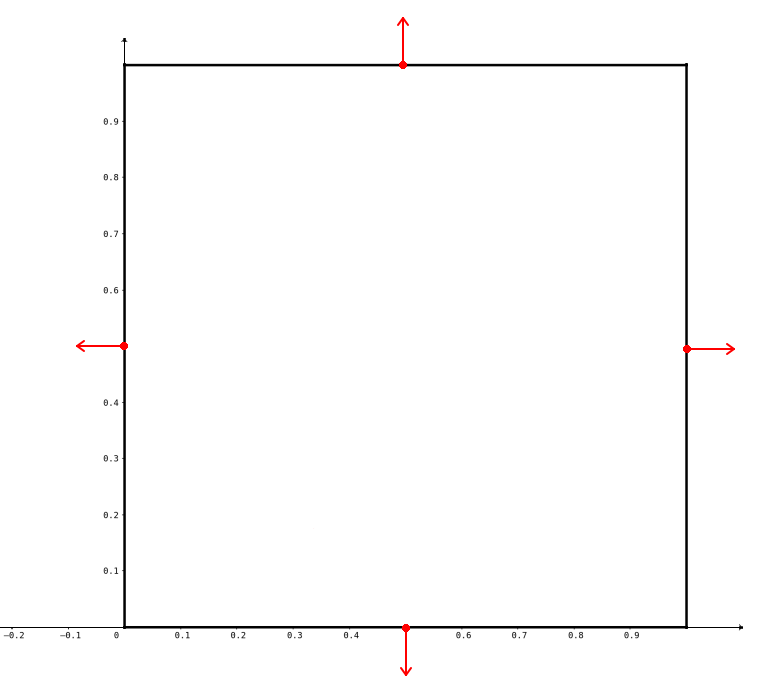
\includegraphics[keepaspectratio, width = 0.55\textwidth]{geomSquare.png}
    \caption{The $4$ normal vectors of the edges of the computational domain for the $2-$dimensional test case, needed for the calculation of the explicit form of Neumann boundary functions}
        \label{geomSquare}
\end{figure}
\begin{figure}[H]
    \centering
    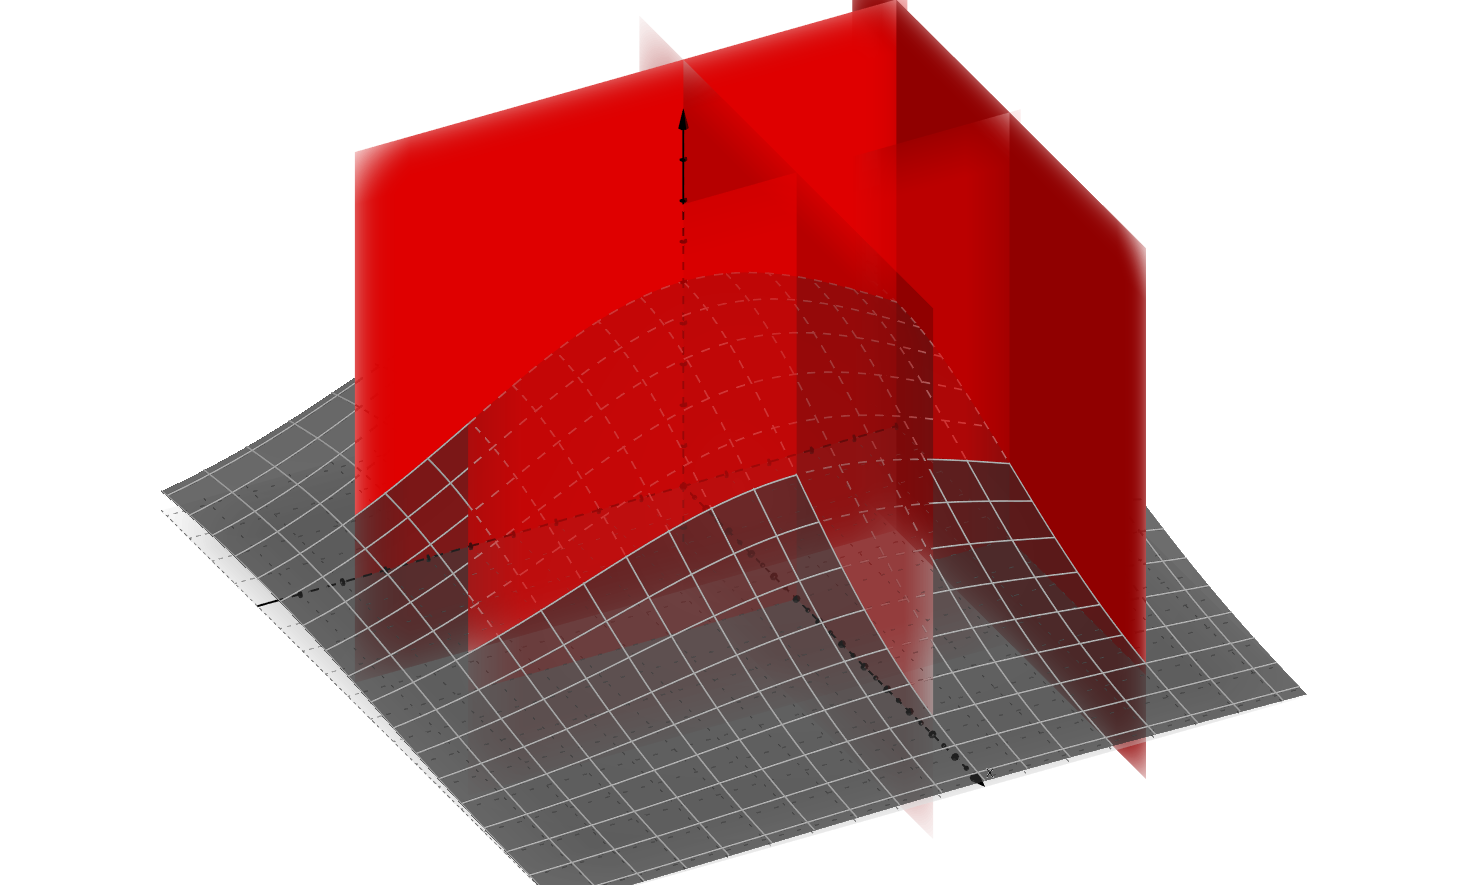
\includegraphics[keepaspectratio, width = \textwidth]{geomSolPlanes.png}
    \caption{The $4$ orthogonal planes to each edge of the computational domain for the $2-$dimensional test case and the projected solution, needed for the calculation of the explicit form of Dirichlet boundary functions}
    \label{geomSolPlanes}
\end{figure}

\newpage
\section{FEM1D}
We will show the application of the $1-$dimensional FEM-based solvers of \code{DiSMA} to our test case.
\subsection{Sim1: stationary uniform diffusion with Dirichlet BCs}
\subsubsection{Sim1.1: results with $\mathbb{P}_1-$basis functions}
\subsubsection{Sim1.2: results with $\mathbb{P}_2-$basis functions}
\subsection{Sim2: stationary uniform diffusion with mixed BCs}
\subsubsection{Sim2.1: results with $\mathbb{P}_1-$basis functions}
\subsubsection{Sim2.2: results with $\mathbb{P}_2-$basis functions}

\newpage
\section{FEM2D}
Here we perform $2-$simulations for the test case with the application \code{FEM2D}, the FEM-based solvers of \code{DiSMA} for planar, rectangular domains using $\mathbb{P}_1$ and $\mathbb{P}_2$ basis functions.
\subsection{Sim3: stationary uniform diffusion with Dirichlet BCs}
We set $\nu(\mathbf{x}) = 1$ throughout the entirety of $\Omega$ which implies that it has null gradient everywhere in the spatial domain. From $(\ref{eq1})$ we immediately notice that only the solution's laplacian term is non-zero and as such we calculate the source function accordingly
\begin{equation*}
    f(\mathbf{x}) = -4(x^2 + y^2 -1)e^{\:\frac{1}{2}\mathbf{x}^T\mathbf{x}} = -4(x^2 + y^2 -1)\,u(\mathbf{x}) \,.
\end{equation*}
Finally we assign the non-homogeneous Dirichlet BCs we derived in \textbf{1.3.2} to all four edges of $\partial\Omega$.

\subsubsection{Sim3.1: results with $\mathbb{P}_1-$basis functions}

\begin{figure}[H]
    \centering
    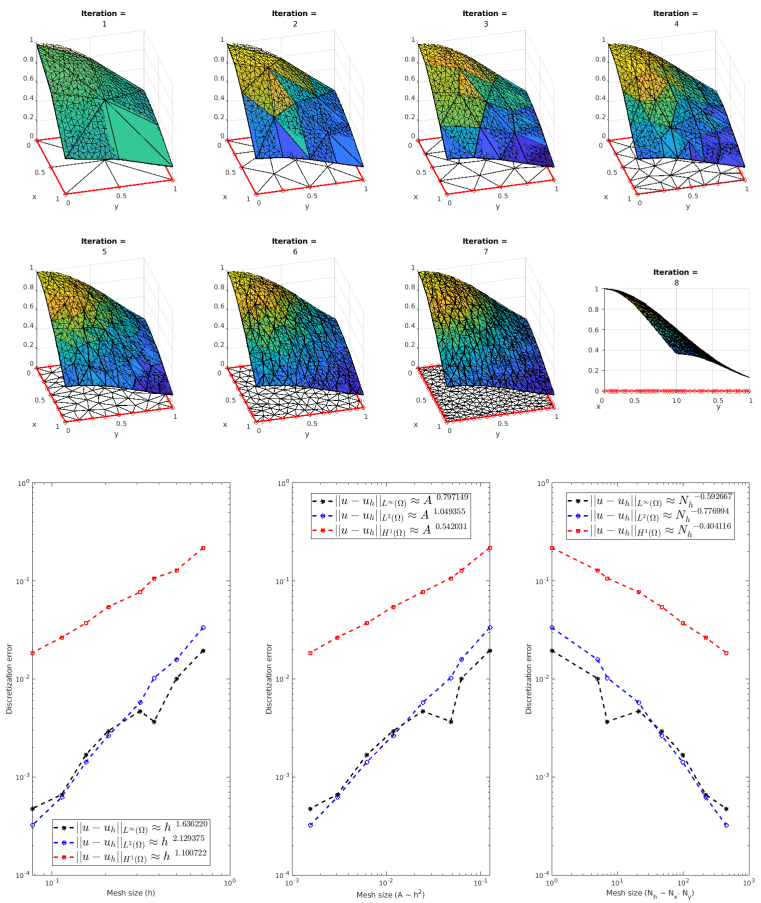
\includegraphics[keepaspectratio,height=0.675\textheight]{sim3.1.png}
    \label{sim3.1}
\end{figure}

\subsubsection{Sim3.2: results with $\mathbb{P}_2-$basis functions}

\begin{figure}[H]
    \centering
    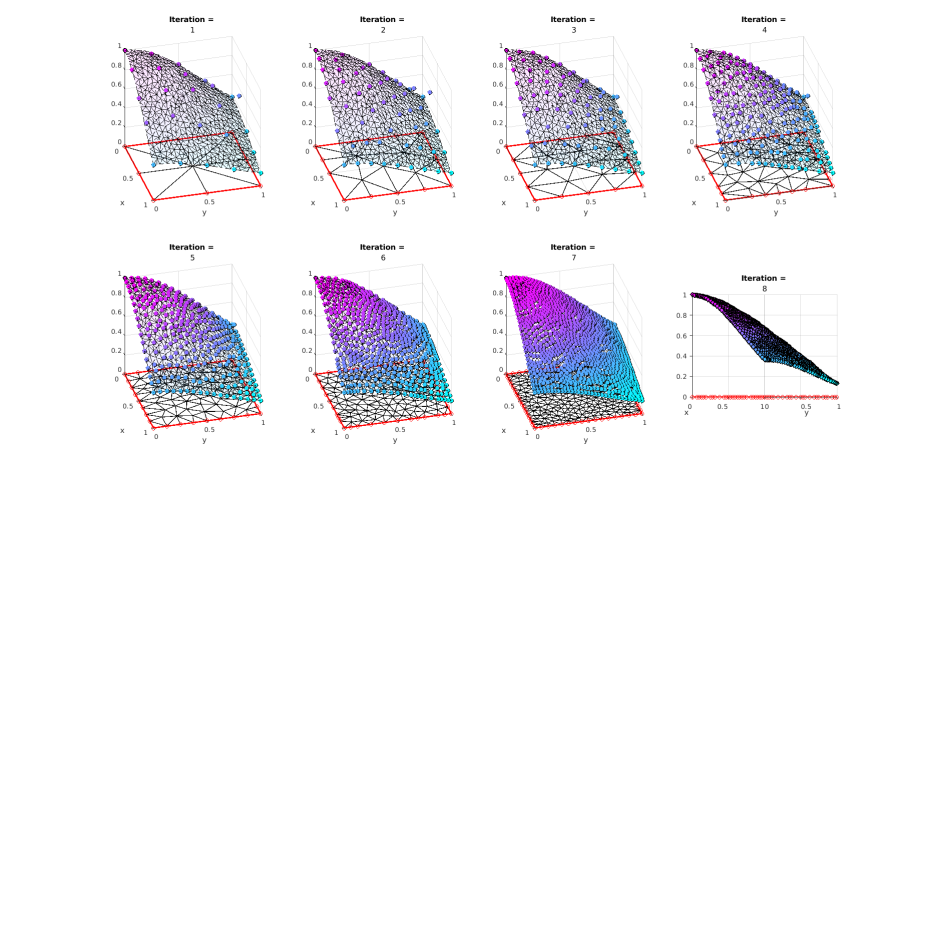
\includegraphics[keepaspectratio,height=0.675\textheight]{sim3.2.png}
    \label{sim3.2}
\end{figure}

\newpage
\subsection{Sim4: stationary uniform diffusion with mixed BCs}
We keep the same value for $\nu$ as in \textbf{Sim3} and as such the source function stays unchanged. The assigned BCs this time however will be Dirichlet's on edges $1$ and $4$ and Neumann's on edges $2$ and $3$ of the border.

\subsubsection{Sim4.1: results with $\mathbb{P}_1-$basis functions}

\begin{figure}[H]
    \centering
    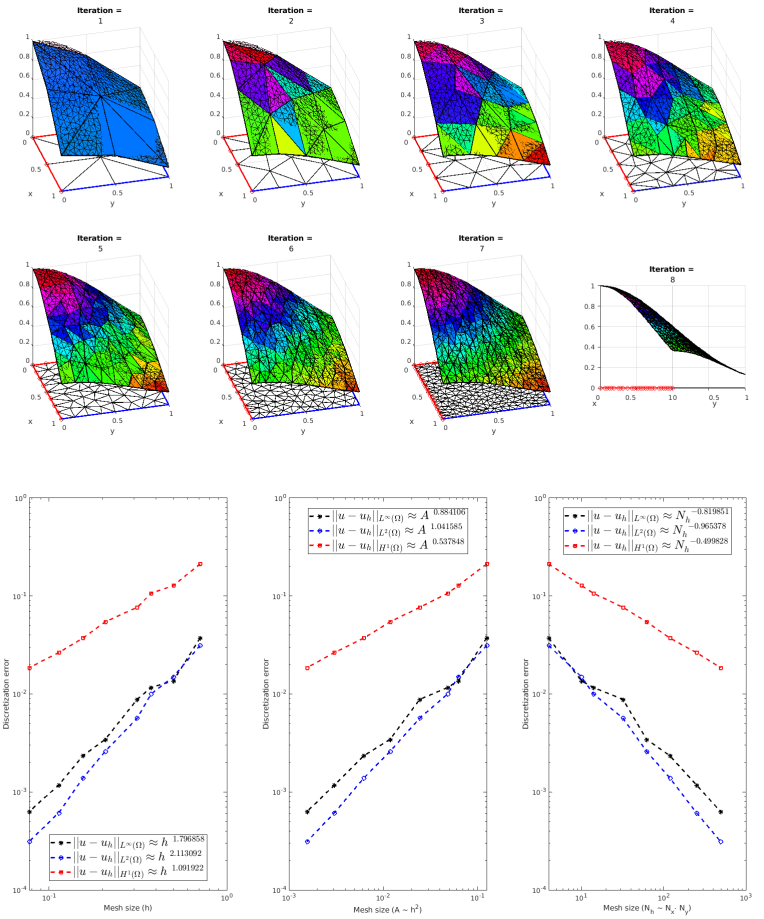
\includegraphics[keepaspectratio,height=0.675\textheight]{sim4.1.png}
    \label{sim4.1}
\end{figure}

\newpage
\subsubsection{Sim4.2: results with $\mathbb{P}_2-$basis functions}

\begin{figure}[H]
    \centering
    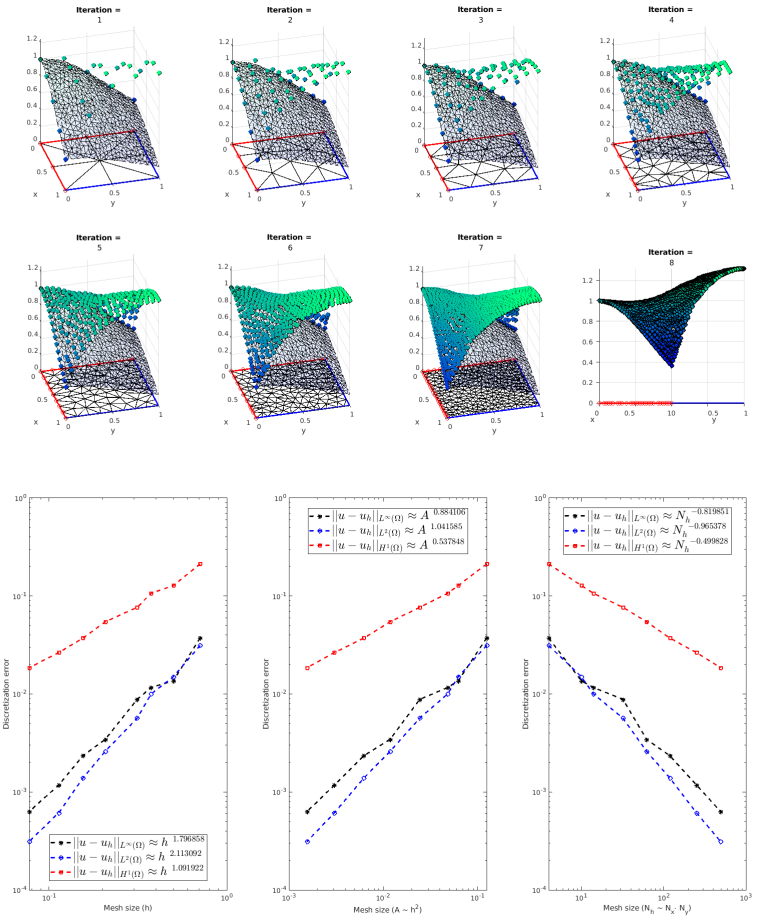
\includegraphics[keepaspectratio,height=0.675\textheight]{sim4.2.png}
    \label{sim4.2}
\end{figure}

\subsection{Sim5: stationary non-uniform diffusion}
Here instead we choose a non-uniform spatial distribution for the diffusion $\nu(\mathbf{x}) = y\sin(x) + x\cos(y) \,,\;\;\forall\mathbf{x}=(x,y)^T\in\Omega$.
As opposed to \textbf{Sim3} here the gradient of $\nu$ is not zero
\begin{equation*}
    \nabla\nu = (\partial_x\nu,\partial_y\nu)^T=(y\cos(x)+\cos(y)\,,\:\sin(x)-x\sin(y))\,,
\end{equation*}
and thus the source function will contain the contributions from both the first the second term in $(\ref{eq1})$ as derived below
\newpage
\begin{align*}
    f(\mathbf{x}) &= 2xy\,\bigg(\cos(x) + \frac{\nu(\mathbf{x})}{xy} - \sin(y)\bigg)u(\mathbf{x}) - 4(x^2 + y^2 -1)\nu(\mathbf{x})\,u(\mathbf{x}) = \\
    &= 2xy\,\bigg(\cos(x) + \frac{\nu(\mathbf{x})}{xy}-2\nu(\mathbf{x})(x^2 + y^2 -1)-\sin(y)\bigg)\,u(\mathbf{x})\,.
\end{align*}
For the BCs we retain the same non-homogeneous Dirichlet BCs set in \textbf{Sim3} for the sake of simplicity.

\subsubsection{Sim5.1: results with $\mathbb{P}_1-$basis functions}

\begin{figure}[H]
    \centering
    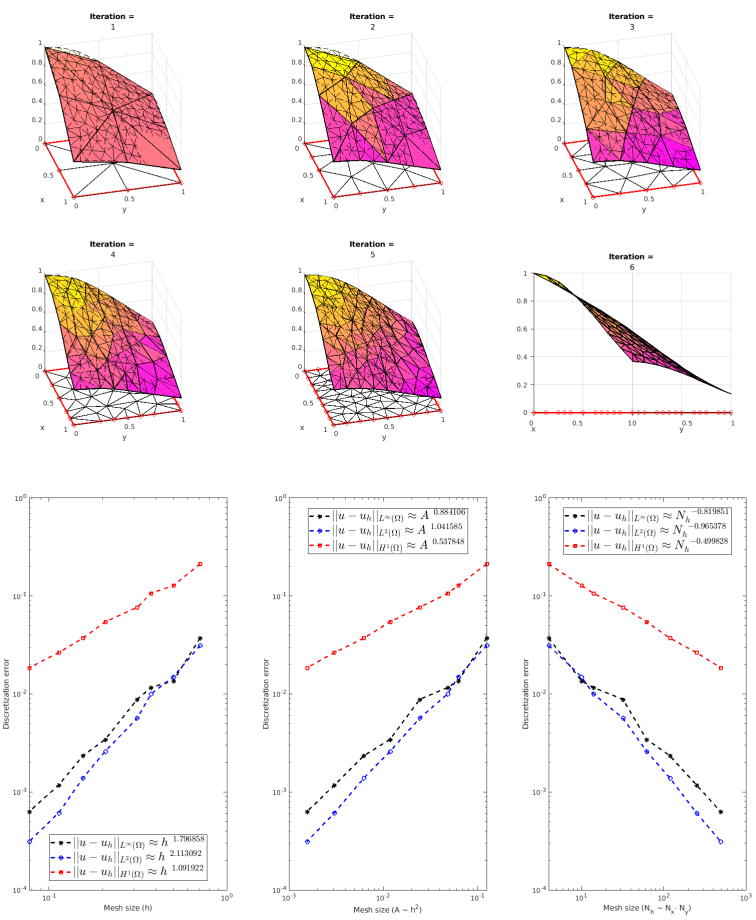
\includegraphics[keepaspectratio,height=0.675\textheight]{sim5.1.png}
    \label{sim5.1}
\end{figure}

\newpage
\subsubsection{Sim5.2: results with $\mathbb{P}_2-$basis functions}

\begin{figure}[H]
    \centering
    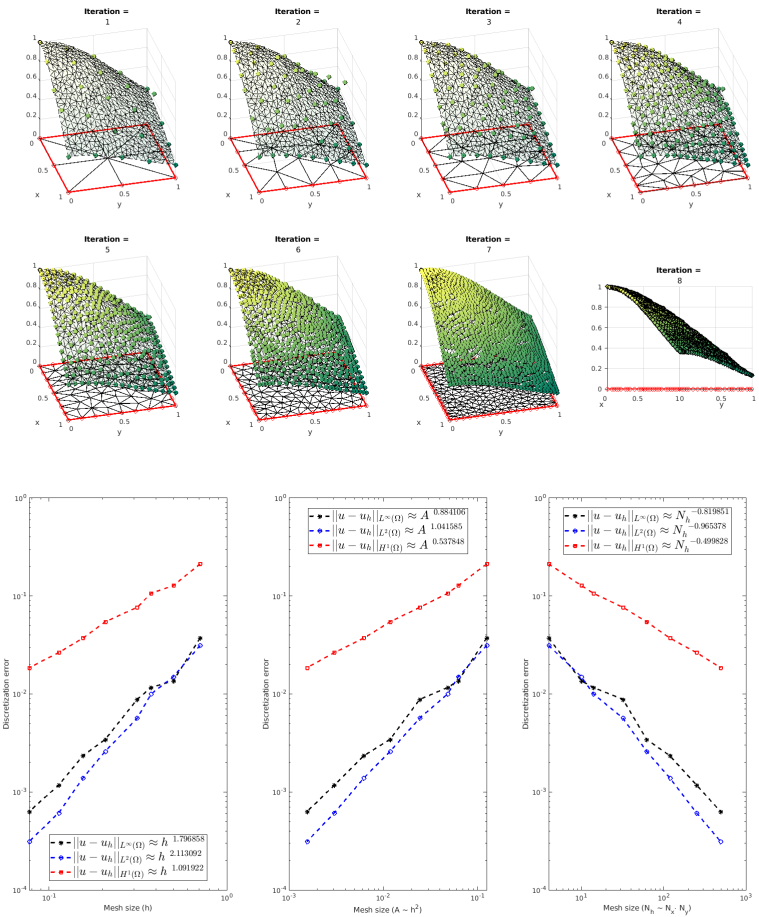
\includegraphics[keepaspectratio,height=0.675\textheight]{sim5.2.png}
    \label{sim5.2}
\end{figure}

\newpage
\subsection{Sim6: unsteady problem with transient diffusion}
As a case-test for a transient solution (one whose time behaviour starts with an initial oscillations that get dumped until a stationary state it's reached) we build the time-dependence for $u(\mathbf{x},t)$ in the following way.
%% Scegliere la diffusione con un decadimento asintotico per dimostrare che passato il transiente dinamico la soluzione si stabilizza ad una stazionaria
\subsubsection{Sim6.1: results with $\mathbb{P}_1-$basis functions}
\subsubsection{Sim6.2: results with $\mathbb{P}_2-$basis functions}

\cleardoublepage
\section{Introduction and motivation}
Different techniques exist in numerical analysis to discretise and solve partial differential equations (PDEs). Among the most widespread we surely find the Finite Element Method (FEM) based on the construction of an ad-hoc finite-dimensional space whose basis is used to linearly derive the approximated solution of a given boundary value (partial) differential problem (IBVP).
\newline In the following we shall address the main features of the aforementioned numerical method by implementing the algorithm on different IBVPs and post-processing its results by evaluating the performances and the accuracy of the former.
\subsection{Variational (weak) formulation: Galerkin's problem}
We shall hereby outline the fundamental assumptions in order for the FEM to converge to the desired solution as well as define the notation and terminology that will be used in the following sections.

\begin{defn}\label{d1}
Let $d\in\mathbb{N}$ be an integer strictly greater than $0$ defining the dimensionality of the PDE , $\Omega\subset\mathbb{R}^d$ be a compact subset and $V$ an Hilbert space with functions valued in $\Omega$ then we define
\begin{equation*}
    \text{find} \: u\in V \;\text{s.t.}\;\: a(u,v)=F(v)\,,\:\forall v\in V
\end{equation*}
a (abstract) variational problem on $\Omega$.
\end{defn}

\begin{theom}\label{t1}
Let $a(u,v)=F(v)$ be a variational problem on a Hilbert space $V$ with $a:V\times V\mapsto\mathbb{R}$ and $F:V\mapsto\mathbb{R}$ some bi-linear and linear forms on $V$ respectively. If $a,\,F$ are s.t.
\begin{itemize}
    \item they verify \textbf{Lax-Milgram theorem};
    \item they depend continuously on the data in $V$;
\end{itemize} 
then the IBVP associated to $a(u,v)=F(v)$ is a \textbf{well-posed problem} in the sense of Hadamard.
\end{theom}

\begin{theom}\label{t2}
Let $a(u,v)=F(v)$ satisfy \ref{t1} and let $V_h\subset V$ be a (finite-dimensional) subspace of $V$ induced by a discretization of the domain (of "size" $h$) of the IBVP and the choice of a basis. If $V_h$ is s.t.
\begin{itemize}
    \item it satisfies \textbf{Cea's lemma};
    \item it satisfies the consistency hypothesis, i.e.
    \begin{equation*}
        \text{dist}(u,V_h)\to0\,,\;h\to0^+
    \end{equation*}
\end{itemize}
then the discretization is convergent i.e. $||u-u_h||_V\to0\,,\;h\to0^+$, with $u_h$ being the discrete solution derived as a linear combination of the basis functions of $V_h$.
\end{theom}
\newpage
\section{$\mathbb{P}_1$ finite elements}
In the present section we shall impose
\begin{equation*}
    V = \big\{v\in\mathcal{C}(\Omega)\:\;\text{s.t.}\:\; v|_e\in\mathbb{P}_1\,,\:\forall e\in\Omega_h\big\},
\end{equation*}
Let's immediately notice that the continuity condition is a fundamental requirement for the formulation of Galerkin's problem however this condition can be relaxed in different techniques.
\subsection{$1-$dimensional IBVPs}
\begin{defn}\label{d2}
Let $L>0$ be a real number and $I=[0,L]\subset\mathbb{R}^+$ a finite, closed interval (domain); let also $f\in L^2(I)$ be a source function and $\mu,\beta,\sigma\in L^{\infty}(I)$ be coefficients functions, then the following
\begin{equation*}
    \text{find}\;u\in V\;\text{s.t.}
    \begin{cases}
    (Du)(x)=-(\mu(x)u^{'}(x))^{'}+\beta(x)u^{'}(x)+\sigma(x)u(x)=f(x)\,,\;\forall x\in(0,L) \\
    u(0) = g_0 \\
    u(L) = g_L
    \end{cases}
\end{equation*}
is an IBVP that will be henceforth referred to as \textbf{diffusion-advection-reaction equation} (DARe)
\end{defn}
\begin{prop}\label{p1}
The problem defined in \ref{d2} satisfies the hypothesis of \ref{t1} if and only if $\mu,\beta,\sigma$ are (uniformly limited) functions in $I$ s.t.
\begin{itemize}
    \item $\mu(x)\geq\mu_0>0$;
    \item $\beta^{'}$ is limited;
    \item $\sigma-\frac{1}{2}\beta^{'}\geq0$
\end{itemize}
\end{prop}
\begin{exmp}\label{ex1}
Let $L=\pi$, $\mu(x)=\beta(x)=\sigma(x)=1$ and $f=Du$ when $u(x)=sin(nx)$ (this imposes the BCs to be $g_0=g_L=0$). Implement a $\mathbb{P}_1-$based FEs algorithm and verify the convergence of \ref{t2}.
\end{exmp}
\textbf{Solution}
\newline The implementation strategy has been performed by including an outer loop in which the number of FEs (i.e. subintervals) of partition $\mathcal{I}_h$ of subset $I$ doubles at each iteration. In particular we wanted to control the discretization step $h$ through an ad-hoc parametrisation that, at each iteration $k\in\mathbb{N}$ refines $\mathcal{I}_h^{(k)}$ in the following way 
\begin{equation*}
    h^{(k)}=\frac{L}{2^k}=\frac{1}{2}\cdot\frac{L}{2^{k-1}}=\frac{1}{2}\cdot h^{(k-1)}
\end{equation*}
where $L=L-0=\mu(I)$ is the measure of subset $I$. It is trivial to observe that the number of FEs is $N_e:=2^k$, the number of \textsl{DOFs} (inner nodes) is $N_h := N_e-1$ and the total number of nodes is $N:=N_h+2=\dots=N_e+1$.
\newline We clearly see that at the fourth iteration $(k=4)$, with merely $15$ nodes of estimation of $\mathcal{I}_h$ the approximation and its derivative almost identically follow the exact solution, as depicted in the below figure, with the behaviour becoming increasingly unstable with greater values of $n=1,2,\pi,...$
\begin{figure}[H]
    \begin{subfigure}[h]{0.3\textwidth}
        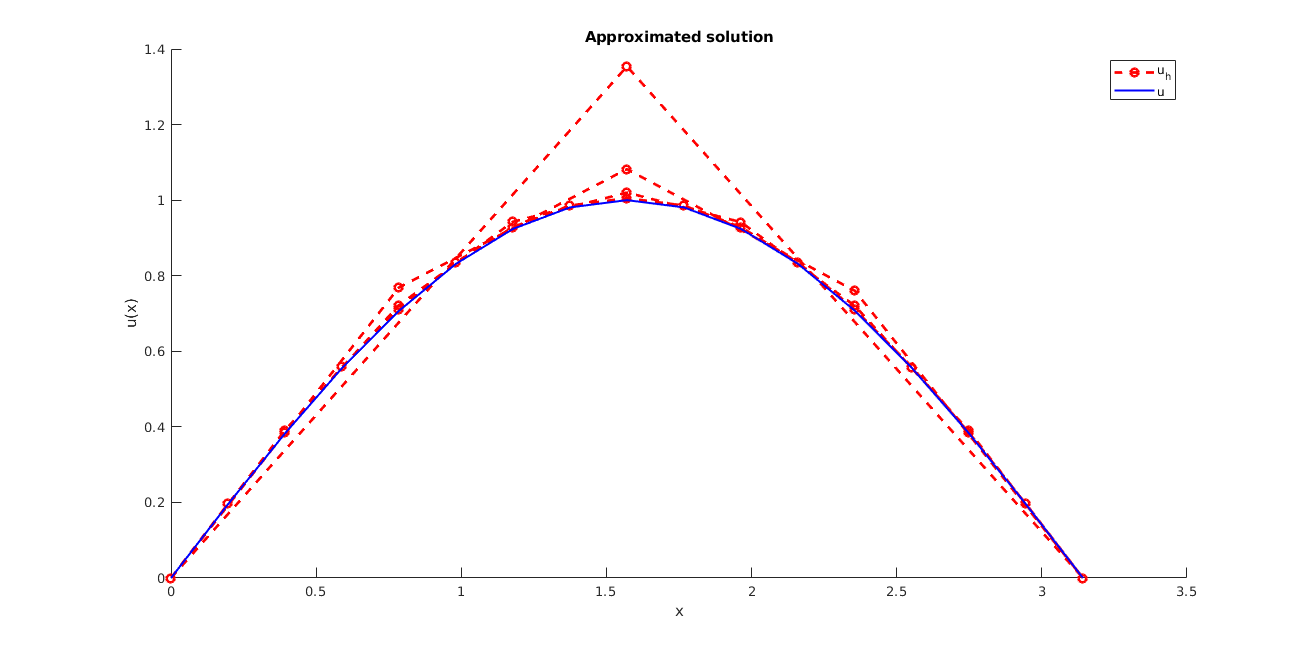
\includegraphics[keepaspectratio,width=6cm]{sinx.png}
    \end{subfigure}
     ~ \;
     \begin{subfigure}[h]{0.3\textwidth}
        %\hspace{-1.15cm}
        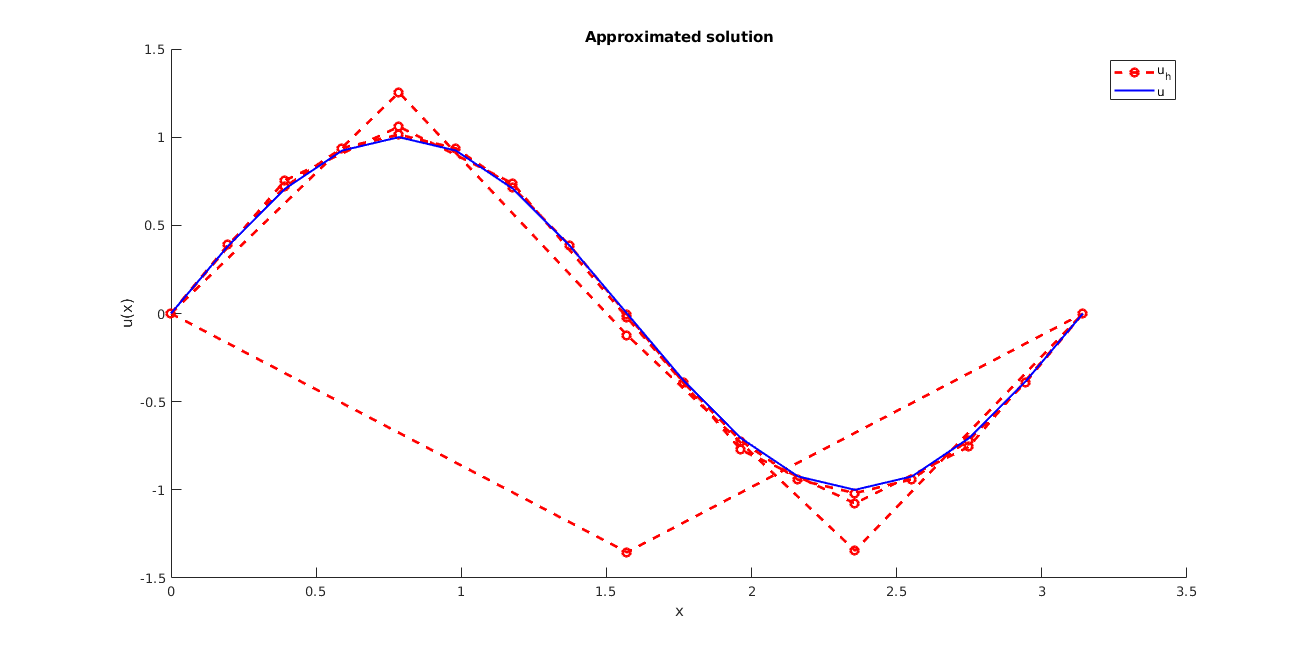
\includegraphics[keepaspectratio,width=6cm]{sin2x.png}
    \end{subfigure}
     ~ \;
     \begin{subfigure}[h]{0.3\textwidth}
        %\hspace{-1.15cm}
        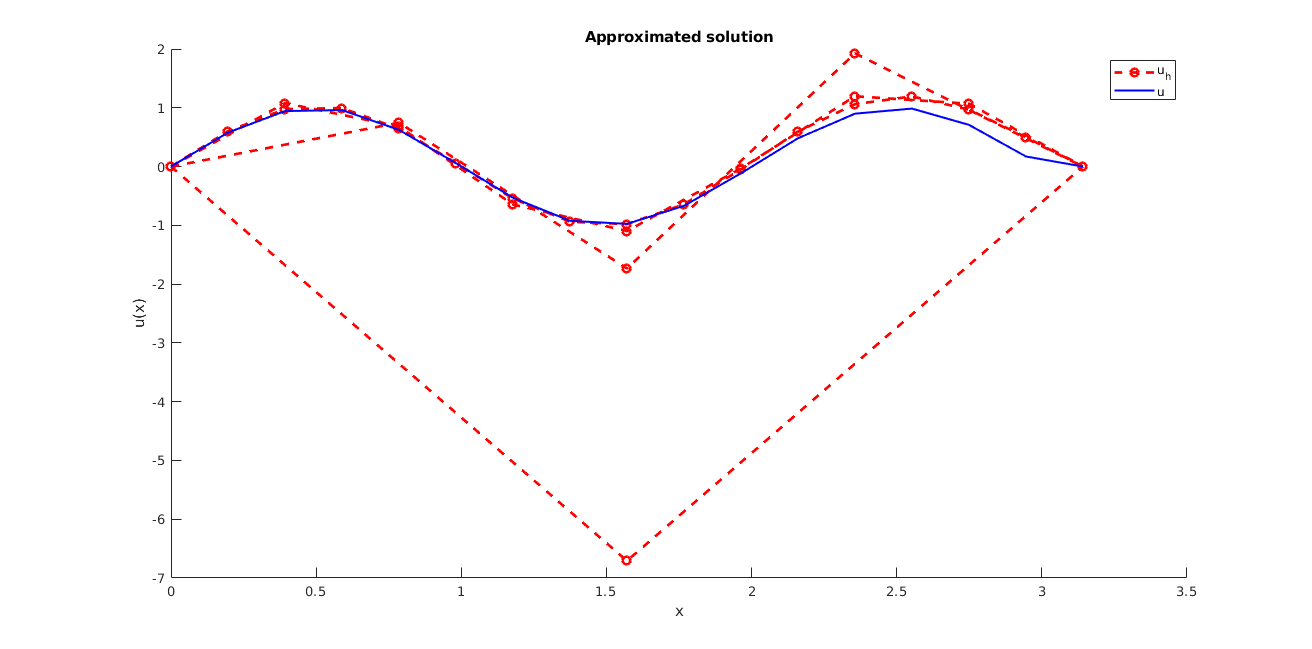
\includegraphics[keepaspectratio,width=6cm]{sinpix.png}
    \end{subfigure}
     \newline
    \begin{subfigure}[h]{0.3\textwidth}
        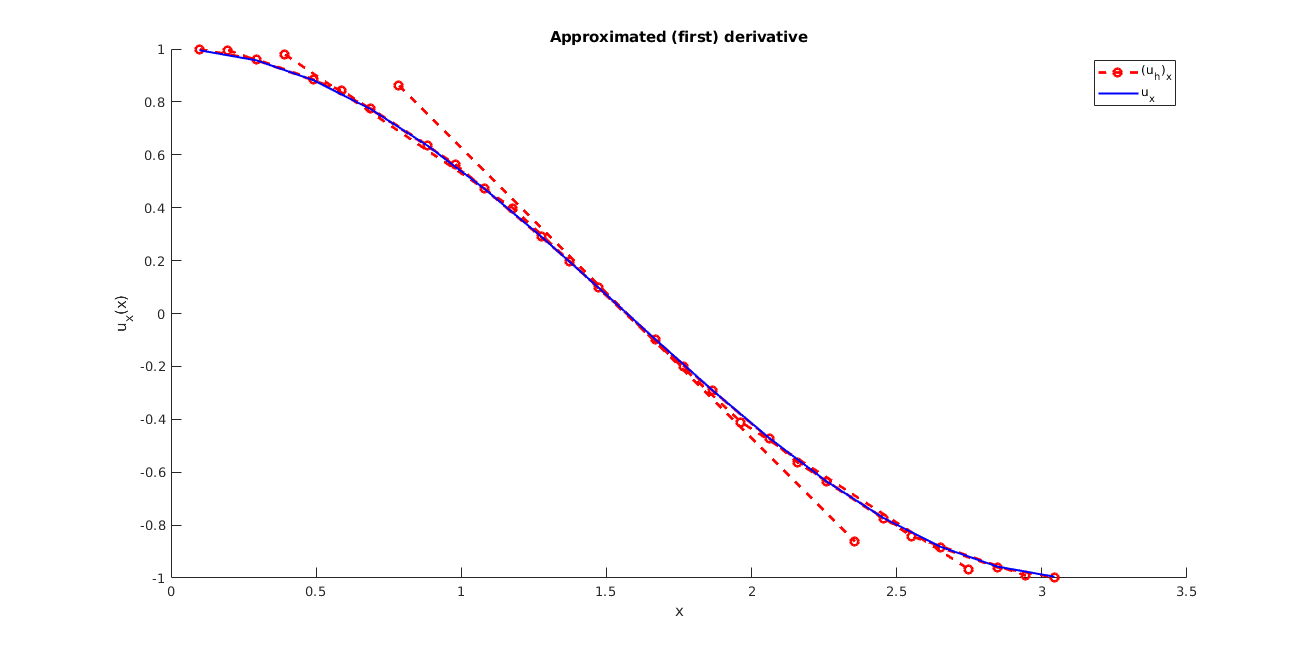
\includegraphics[keepaspectratio,width=6cm]{cosx.png}
    \end{subfigure}
     ~ \;
     \begin{subfigure}[h]{0.3\textwidth}
        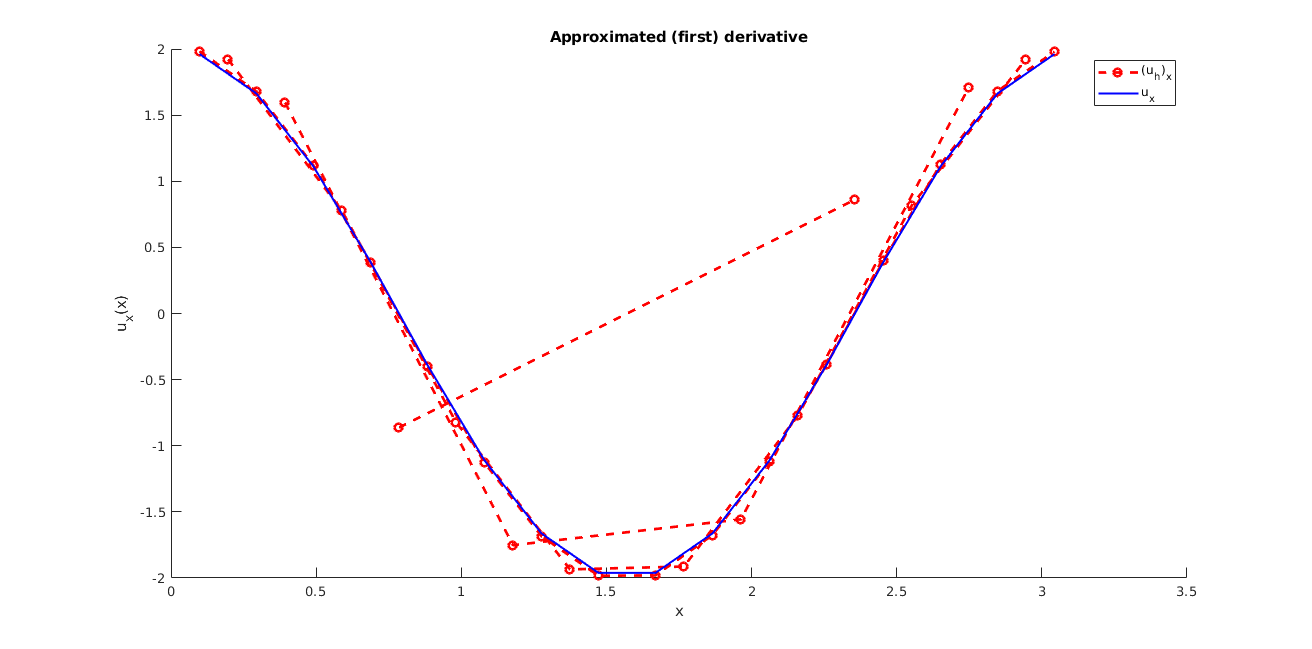
\includegraphics[keepaspectratio,width=6cm]{cos2x.png}
    \end{subfigure}
     ~ \;
     \begin{subfigure}[h]{0.3\textwidth}
        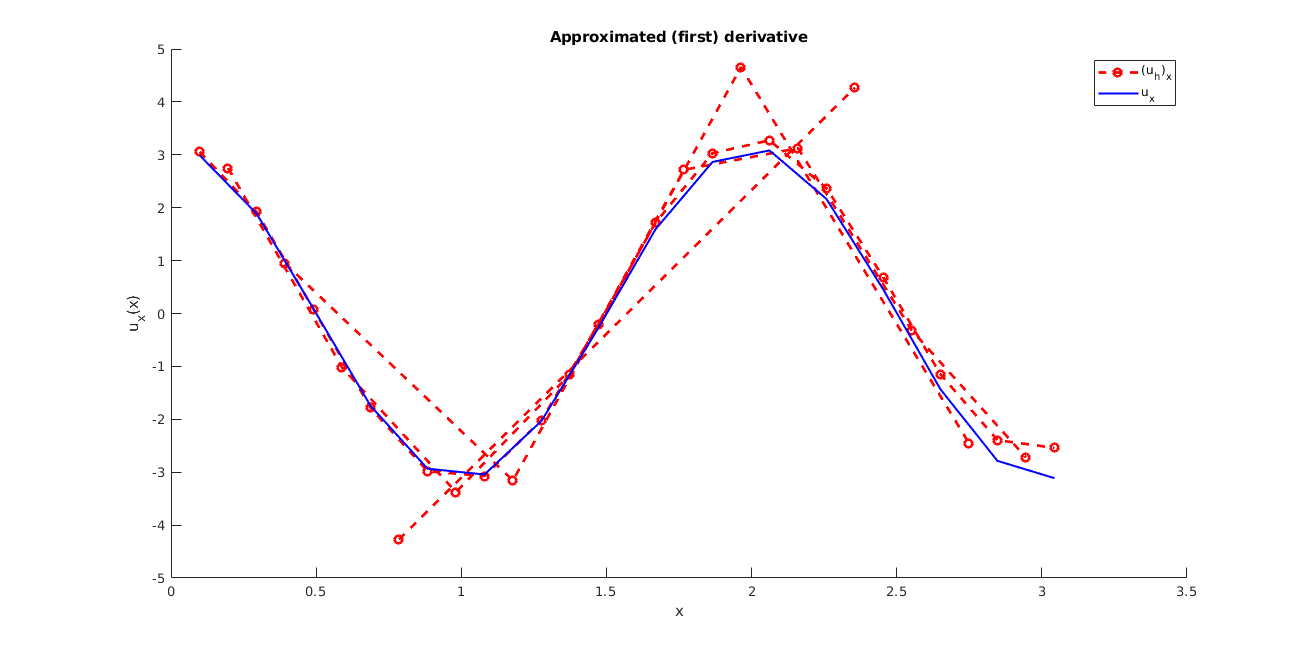
\includegraphics[keepaspectratio,width=6cm]{cospix.png}
    \end{subfigure}
    \captionsetup{singlelinecheck=off}
    \caption{Convergence of the iterative approximations of the FEM solution to the exact solution (first row) and their respective (first order) derivatives (second row). From left to right we have different values of integer $n$ in $sin(nx)$, specifically $n=1$ (leftmost), $n=2$ (centre), $n=\pi$ (rightmost)}
    \label{fig1}
\end{figure}
The instability at greater values of $n$ can be easily evaluated also from the errors' norm estimation, depicted below.
\begin{figure}[H]
    \begin{subfigure}[h]{0.3\textwidth}
        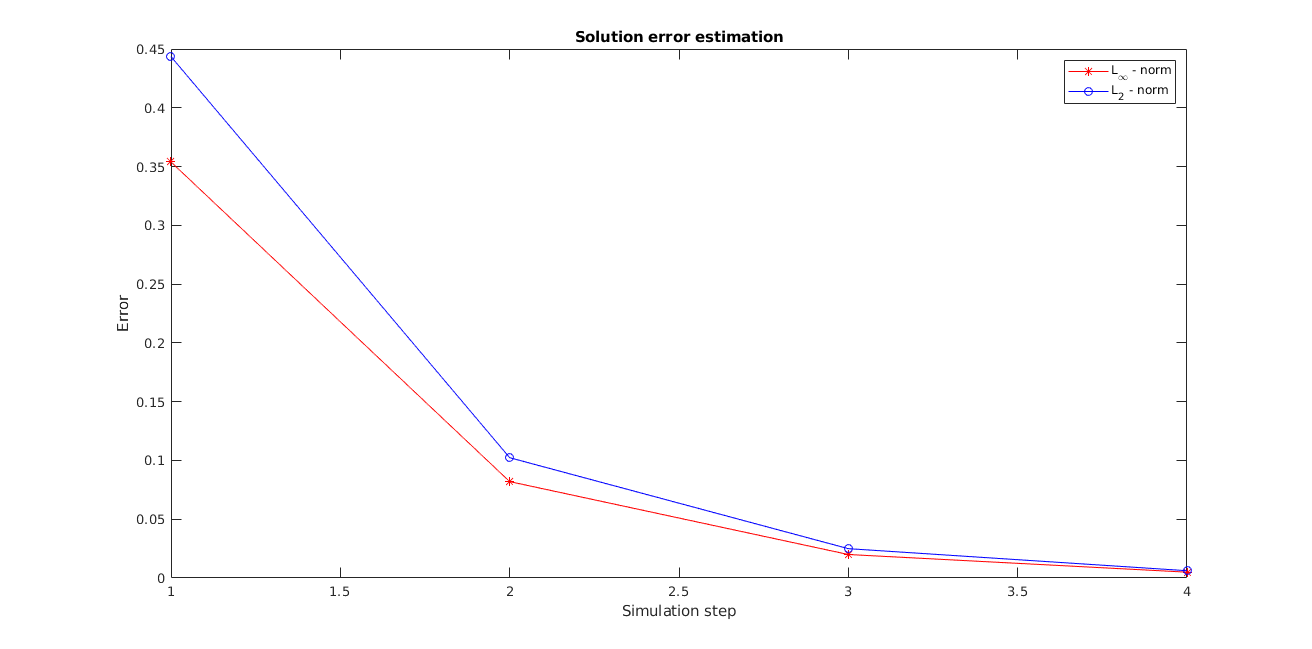
\includegraphics[keepaspectratio,width=6cm]{sinx_error.png}
    \end{subfigure}
     ~ \;
     \begin{subfigure}[h]{0.3\textwidth}
        %\hspace{-1.15cm}
        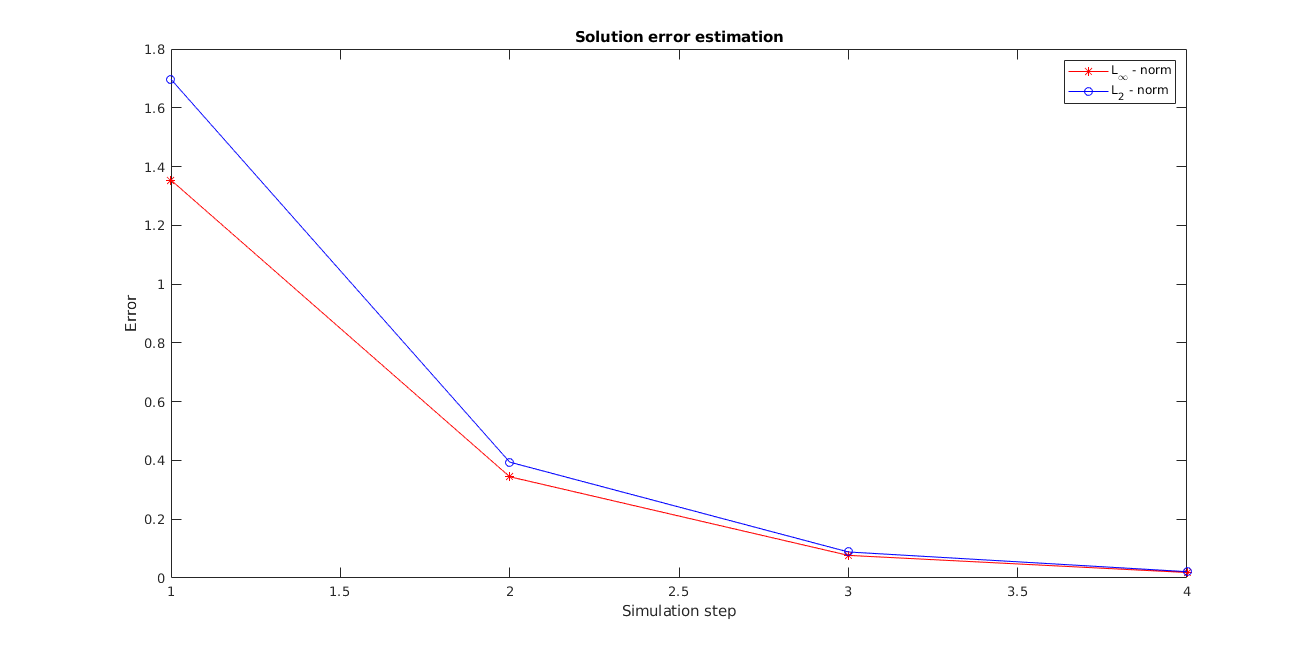
\includegraphics[keepaspectratio,width=6cm]{sin2x_error.png}
    \end{subfigure}
     ~ \;
     \begin{subfigure}[h]{0.3\textwidth}
        %\hspace{-1.15cm}
        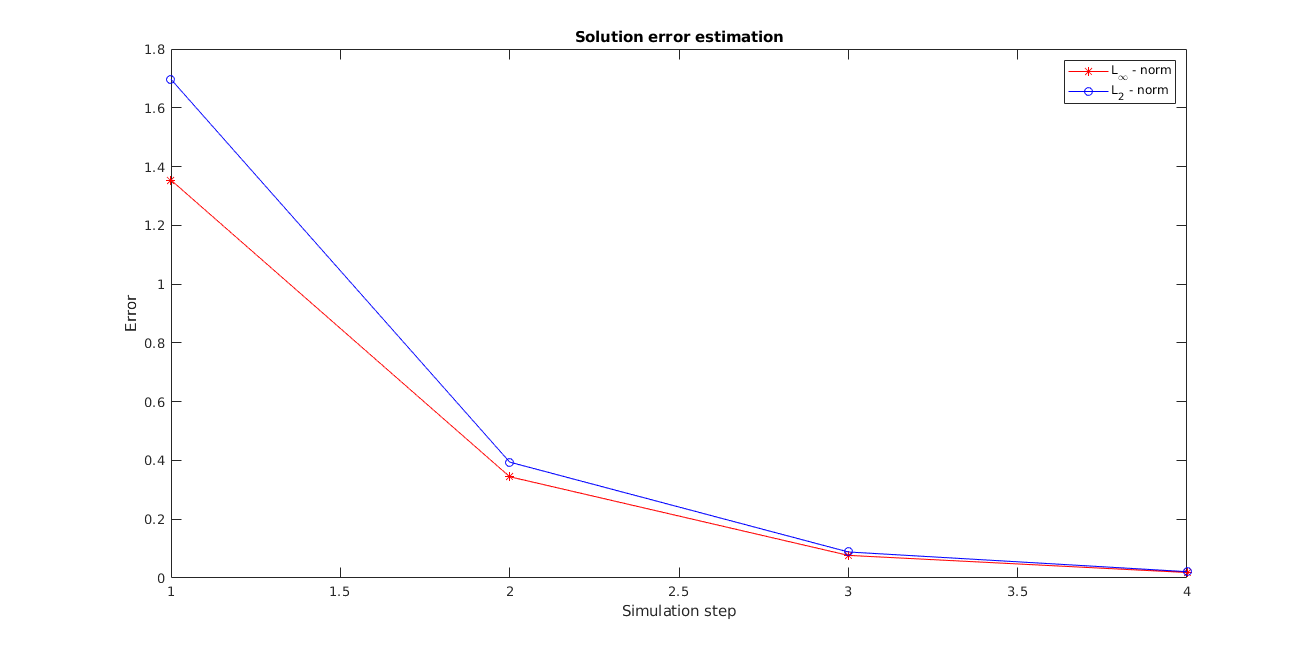
\includegraphics[keepaspectratio,width=6cm]{sinpix_error.png}
    \end{subfigure}
     \newline
    \begin{subfigure}[h]{0.3\textwidth}
        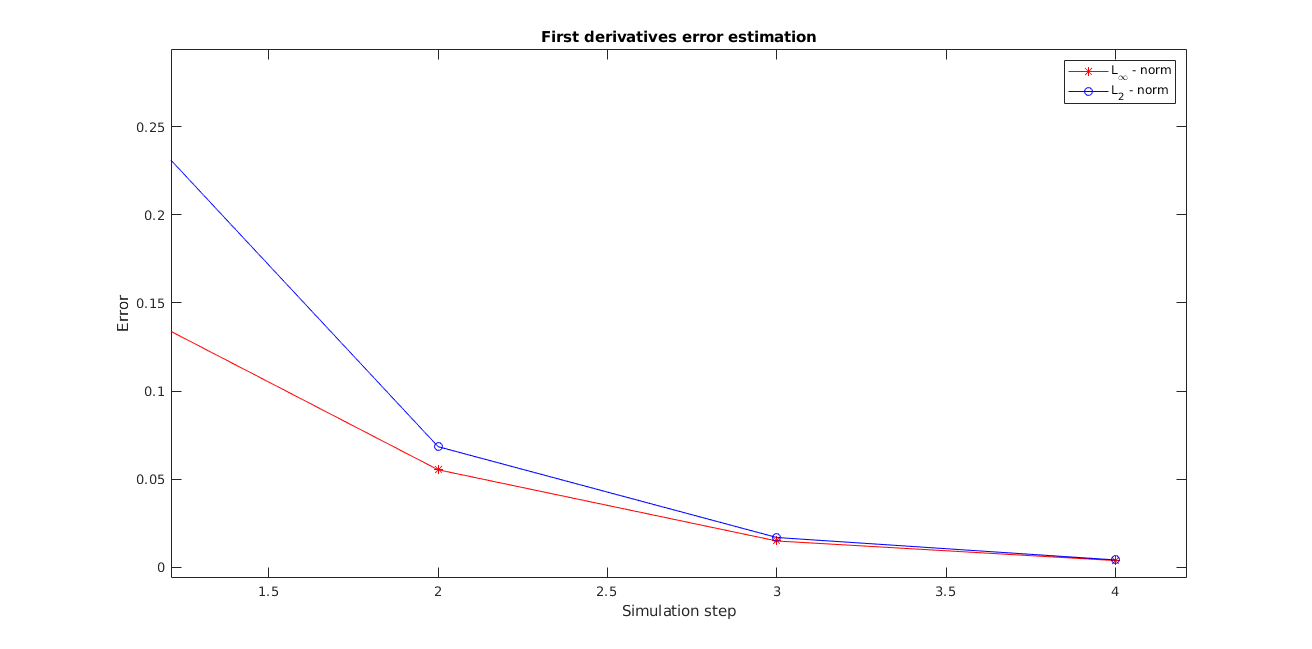
\includegraphics[keepaspectratio,width=6cm]{cosx_error.png}
    \end{subfigure}
     ~ \;
     \begin{subfigure}[h]{0.3\textwidth}
        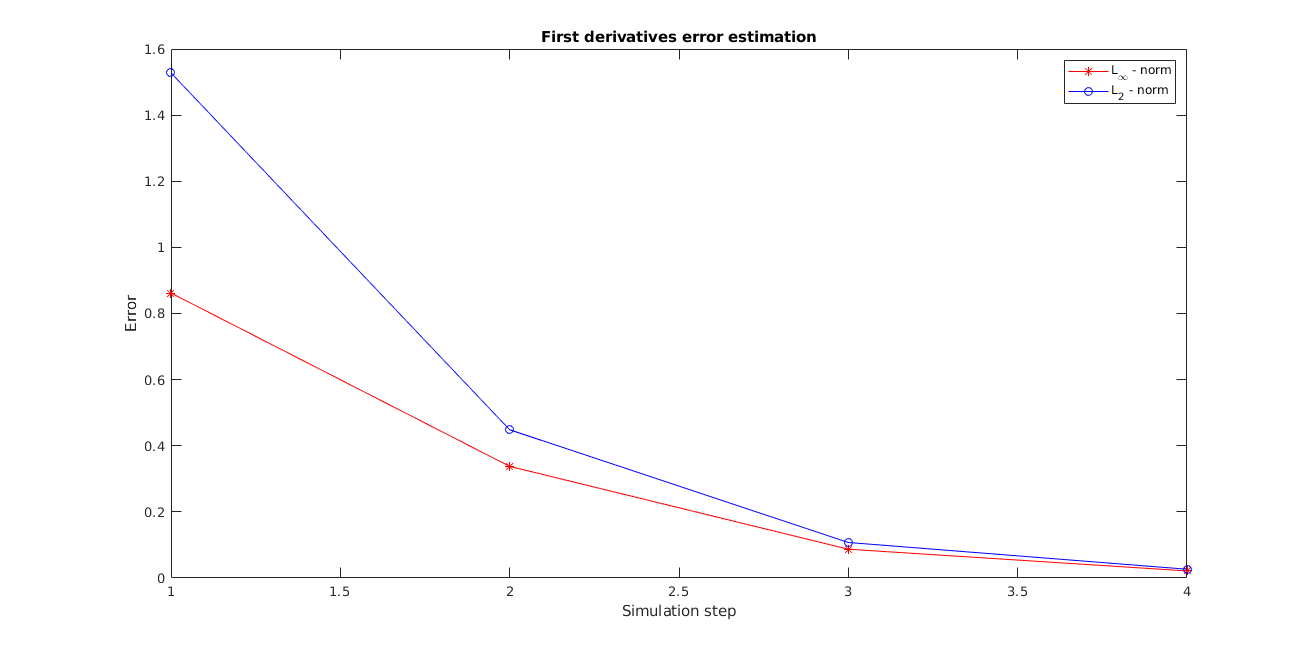
\includegraphics[keepaspectratio,width=6cm]{cos2x_error.png}
    \end{subfigure}
     ~ \;
     \begin{subfigure}[h]{0.3\textwidth}
        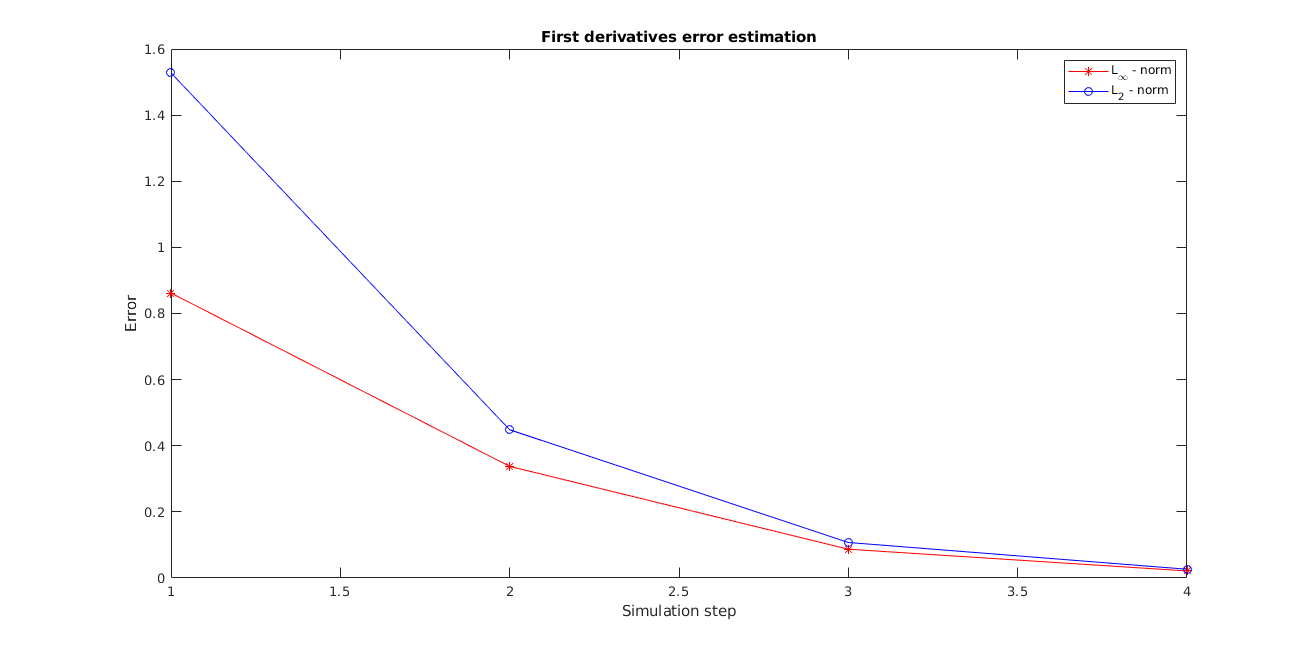
\includegraphics[keepaspectratio,width=6cm]{cospix_error.png}
    \end{subfigure}
    \captionsetup{singlelinecheck=off}
\end{figure}
\newpage
\begin{exmp}\label{ex2}
Let $L=2$, $\mu(x)=1+x, \beta(x)=3x, \sigma(x)=e^x$ and $f=1$ with homogeneous Dirichlet BCs. Estimates the value of the solution of the DARe in $x=1$.
\end{exmp}
\textbf{Solution}
\newline Let's implement the same strategy of \label{ex1} and let's verify the convergence of $u_h$ to $u$. The results are consistent with those of \ref{ex1} as depicted in the following Figure. 
\newline
We conclude that, as of the tenth iteration (i.e. $k=10\Rightarrow N_h=1023$), the estimation of $u(x)$ in x=1 is as follows
\begin{equation*}
    \lim_{h\to0^+}u_h(x=1)=0.1747\approx u(x=1)
\end{equation*}

\begin{figure}[H]
    \begin{subfigure}[H]{0.75\textwidth}
        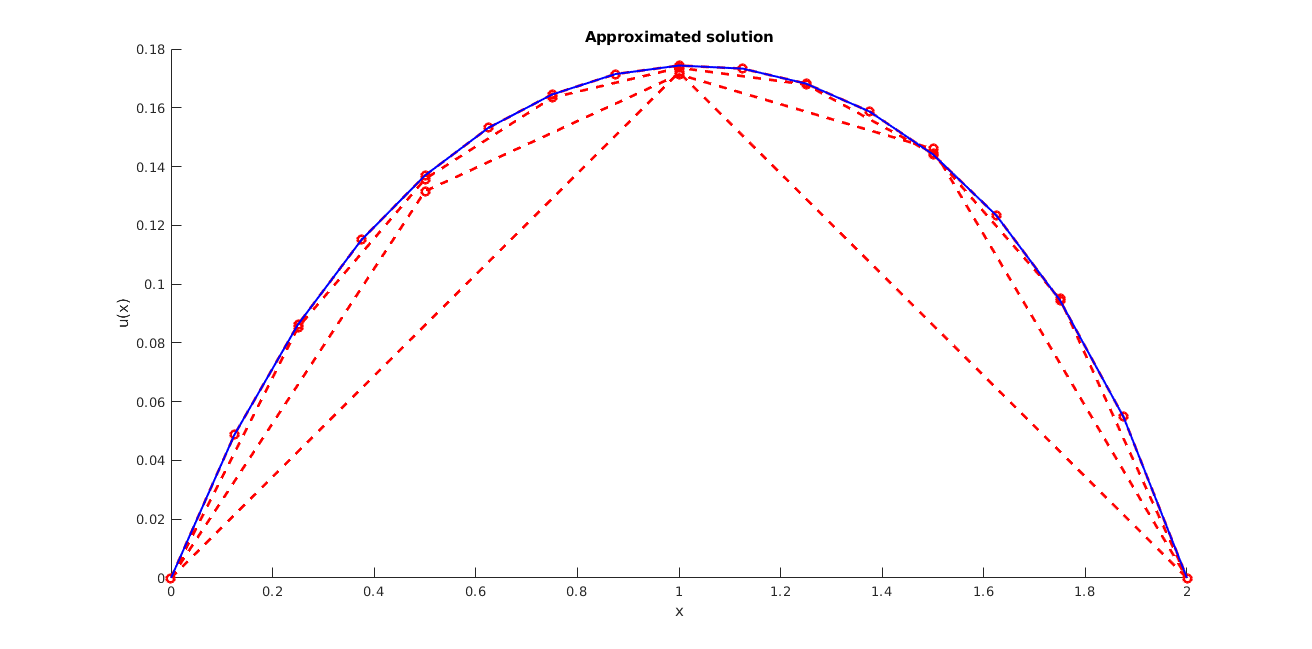
\includegraphics[keepaspectratio,width=1.25\textwidth]{ex2_1.png}
    \end{subfigure}
     \newline
     \begin{subfigure}[H]{0.75\textwidth}
        %\hspace{-1.15cm}
        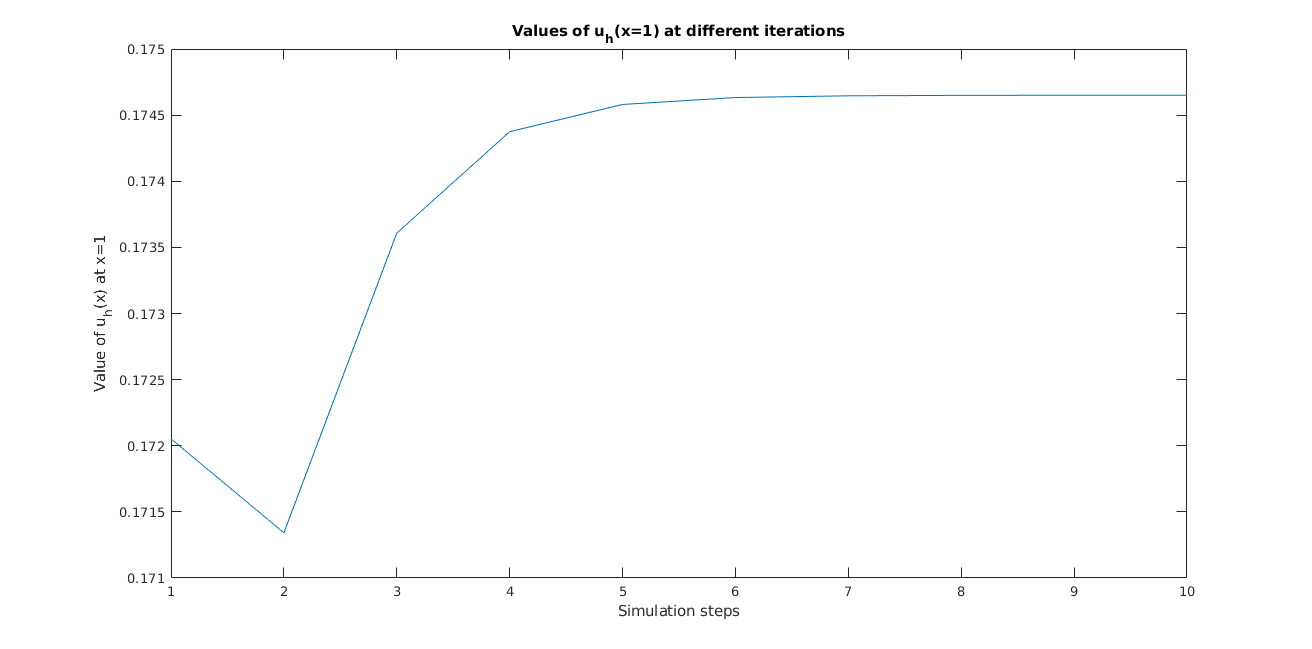
\includegraphics[keepaspectratio,width=\textwidth]{ex2_2.png}
    \end{subfigure}
     \captionsetup{singlelinecheck=off}
     \caption{(Top) Iterative approximations of $u_h^{(k)}$; we can see that it does resemble the same convergence property of \ref{ex1}.\newline(Bottom) Iterative evaluations of $u_h^{(k)}$ in x=1 (midpoint of the computational domain}
\end{figure}
\newpage
\begin{exmp}\label{ex3}
With the same data of \ref{ex2}, but in the case on non-homogeneous BCs $g_0=2\,,\:g_L=5$, Estimates the value of the solution of the DARe in $x=1$.
\end{exmp}
\textbf{Solution}
\newline Following the methodologies laid down in both \ref{ex1} and \ref{ex2} we concluded 
\begin{equation*}
    \lim_{h\to0^+}u_h(x=1)=-1.2856
\end{equation*}
\end{document}
